
%% bare_conf.tex
%% V1.4
%% 2012/12/27
%% by Michael Shell
%% See:
%% http://www.michaelshell.org/
%% for current contact information.
%%
%% This is a skeleton file demonstrating the use of IEEEtran.cls
%% (requires IEEEtran.cls version 1.8 or later) with an IEEE conference paper.
%%
%% Support sites:
%% http://www.michaelshell.org/tex/ieeetran/
%% http://www.ctan.org/tex-archive/macros/latex/contrib/IEEEtran/
%% and
%% http://www.ieee.org/

%%*************************************************************************
%% Legal Notice:
%% This code is offered as-is without any warranty either expressed or
%% implied; without even the implied warranty of MERCHANTABILITY or
%% FITNESS FOR A PARTICULAR PURPOSE! 
%% User assumes all risk.
%% In no event shall IEEE or any contributor to this code be liable for
%% any damages or losses, including, but not limited to, incidental,
%% consequential, or any other damages, resulting from the use or misuse
%% of any information contained here.
%%
%% All comments are the opinions of their respective authors and are not
%% necessarily endorsed by the IEEE.
%%
%% This work is distributed under the LaTeX Project Public License (LPPL)
%% ( http://www.latex-project.org/ ) version 1.3, and may be freely used,
%% distributed and modified. A copy of the LPPL, version 1.3, is included
%% in the base LaTeX documentation of all distributions of LaTeX released
%% 2003/12/01 or later.
%% Retain all contribution notices and credits.
%% ** Modified files should be clearly indicated as such, including  **
%% ** renaming them and changing author support contact information. **
%%
%% File list of work: IEEEtran.cls, IEEEtran_HOWTO.pdf, bare_adv.tex,
%%                    bare_conf.tex, bare_jrnl.tex, bare_jrnl_compsoc.tex,
%%                    bare_jrnl_transmag.tex
%%*************************************************************************

% *** Authors should verify (and, if needed, correct) their LaTeX system  ***
% *** with the testflow diagnostic prior to trusting their LaTeX platform ***
% *** with production work. IEEE's font choices can trigger bugs that do  ***
% *** not appear when using other class files.                            ***
% The testflow support page is at:
% http://www.michaelshell.org/tex/testflow/



% Note that the a4paper option is mainly intended so that authors in
% countries using A4 can easily print to A4 and see how their papers will
% look in print - the typesetting of the document will not typically be
% affected with changes in paper size (but the bottom and side margins will).
% Use the testflow package mentioned above to verify correct handling of
% both paper sizes by the user's LaTeX system.
%
% Also note that the "draftcls" or "draftclsnofoot", not "draft", option
% should be used if it is desired that the figures are to be displayed in
% draft mode.
%
\documentclass[conference]{IEEEtran}
% Add the compsoc option for Computer Society conferences.
%
% If IEEEtran.cls has not been installed into the LaTeX system files,
% manually specify the path to it like:
% \documentclass[conference]{../sty/IEEEtran}


% Some very useful LaTeX packages include:
% (uncomment the ones you want to load)
\usepackage{graphicx}
\usepackage{layouts}
% *** MISC UTILITY PACKAGES ***
%
%\usepackage{ifpdf}
% Heiko Oberdiek's ifpdf.sty is very useful if you need conditional
% compilation based on whether the output is pdf or dvi.
% usage:
% \ifpdf
%   % pdf code
% \else
%   % dvi code
% \fi
% The latest version of ifpdf.sty can be obtained from:
% http://www.ctan.org/tex-archive/macros/latex/contrib/oberdiek/
% Also, note that IEEEtran.cls V1.7 and later provides a builtin
% \ifCLASSINFOpdf conditional that works the same way.
% When switching from latex to pdflatex and vice-versa, the compiler may
% have to be run twice to clear warning/error messages.



% *** CITATION PACKAGES ***
%
\usepackage{cite}
% cite.sty was written by Donald Arseneau
% V1.6 and later of IEEEtran pre-defines the format of the cite.sty package
% \cite{} output to follow that of IEEE. Loading the cite package will
% result in citation numbers being automatically sorted and properly
% "compressed/ranged". e.g., [1], [9], [2], [7], [5], [6] without using
% cite.sty will become [1], [2], [5]--[7], [9] using cite.sty. cite.sty's
% \cite will automatically add leading space, if needed. Use cite.sty's
% noadjust option (cite.sty V3.8 and later) if you want to turn this off
% such as if a citation ever needs to be enclosed in parenthesis.
% cite.sty is already installed on most LaTeX systems. Be sure and use
% version 4.0 (2003-05-27) and later if using hyperref.sty. cite.sty does
% not currently provide for hyperlinked citations.
% The latest version can be obtained at:
% http://www.ctan.org/tex-archive/macros/latex/contrib/cite/
% The documentation is contained in the cite.sty file itself.


% *** MATH PACKAGES ***
%
%\usepackage[cmex10]{amsmath}
% A popular package from the American Mathematical Society that provides
% many useful and powerful commands for dealing with mathematics. If using
% it, be sure to load this package with the cmex10 option to ensure that
% only type 1 fonts will utilized at all point sizes. Without this option,
% it is possible that some math symbols, particularly those within
% footnotes, will be rendered in bitmap form which will result in a
% document that can not be IEEE Xplore compliant!
%
% Also, note that the amsmath package sets \interdisplaylinepenalty to 10000
% thus preventing page breaks from occurring within multiline equations. Use:
%\interdisplaylinepenalty=2500
% after loading amsmath to restore such page breaks as IEEEtran.cls normally
% does. amsmath.sty is already installed on most LaTeX systems. The latest
% version and documentation can be obtained at:
% http://www.ctan.org/tex-archive/macros/latex/required/amslatex/math/


% *** SPECIALIZED LIST PACKAGES ***
%
%\usepackage{algorithmic}
% algorithmic.sty was written by Peter Williams and Rogerio Brito.
% This package provides an algorithmic environment fo describing algorithms.
% You can use the algorithmic environment in-text or within a figure
% environment to provide for a floating algorithm. Do NOT use the algorithm
% floating environment provided by algorithm.sty (by the same authors) or
% algorithm2e.sty (by Christophe Fiorio) as IEEE does not use dedicated
% algorithm float types and packages that provide these will not provide
% correct IEEE style captions. The latest version and documentation of
% algorithmic.sty can be obtained at:
% http://www.ctan.org/tex-archive/macros/latex/contrib/algorithms/
% There is also a support site at:
% http://algorithms.berlios.de/index.html
% Also of interest may be the (relatively newer and more customizable)
% algorithmicx.sty package by Szasz Janos:
% http://www.ctan.org/tex-archive/macros/latex/contrib/algorithmicx/




% *** ALIGNMENT PACKAGES ***
%
%\usepackage{array}
% Frank Mittelbach's and David Carlisle's array.sty patches and improves
% the standard LaTeX2e array and tabular environments to provide better
% appearance and additional user controls. As the default LaTeX2e table
% generation code is lacking to the point of almost being broken with
% respect to the quality of the end results, all users are strongly
% advised to use an enhanced (at the very least that provided by array.sty)
% set of table tools. array.sty is already installed on most systems. The
% latest version and documentation can be obtained at:
% http://www.ctan.org/tex-archive/macros/latex/required/tools/


% IEEEtran contains the IEEEeqnarray family of commands that can be used to
% generate multiline equations as well as matrices, tables, etc., of high
% quality.




% *** SUBFIGURE PACKAGES ***
%\ifCLASSOPTIONcompsoc
%  \usepackage[caption=false,font=normalsize,labelfont=sf,textfont=sf]{subfig}
%\else
%  \usepackage[caption=false,font=footnotesize]{subfig}
%\fi
% subfig.sty, written by Steven Douglas Cochran, is the modern replacement
% for subfigure.sty, the latter of which is no longer maintained and is
% incompatible with some LaTeX packages including fixltx2e. However,
% subfig.sty requires and automatically loads Axel Sommerfeldt's caption.sty
% which will override IEEEtran.cls' handling of captions and this will result
% in non-IEEE style figure/table captions. To prevent this problem, be sure
% and invoke subfig.sty's "caption=false" package option (available since
% subfig.sty version 1.3, 2005/06/28) as this is will preserve IEEEtran.cls
% handling of captions.
% Note that the Computer Society format requires a larger sans serif font
% than the serif footnote size font used in traditional IEEE formatting
% and thus the need to invoke different subfig.sty package options depending
% on whether compsoc mode has been enabled.
%
% The latest version and documentation of subfig.sty can be obtained at:
% http://www.ctan.org/tex-archive/macros/latex/contrib/subfig/




% *** FLOAT PACKAGES ***
%
%\usepackage{fixltx2e}
% fixltx2e, the successor to the earlier fix2col.sty, was written by
% Frank Mittelbach and David Carlisle. This package corrects a few problems
% in the LaTeX2e kernel, the most notable of which is that in current
% LaTeX2e releases, the ordering of single and double column floats is not
% guaranteed to be preserved. Thus, an unpatched LaTeX2e can allow a
% single column figure to be placed prior to an earlier double column
% figure. The latest version and documentation can be found at:
% http://www.ctan.org/tex-archive/macros/latex/base/


%\usepackage{stfloats}
% stfloats.sty was written by Sigitas Tolusis. This package gives LaTeX2e
% the ability to do double column floats at the bottom of the page as well
% as the top. (e.g., "\begin{figure*}[!b]" is not normally possible in
% LaTeX2e). It also provides a command:
%\fnbelowfloat
% to enable the placement of footnotes below bottom floats (the standard
% LaTeX2e kernel puts them above bottom floats). This is an invasive package
% which rewrites many portions of the LaTeX2e float routines. It may not work
% with other packages that modify the LaTeX2e float routines. The latest
% version and documentation can be obtained at:
% http://www.ctan.org/tex-archive/macros/latex/contrib/sttools/
% Do not use the stfloats baselinefloat ability as IEEE does not allow
% \baselineskip to stretch. Authors submitting work to the IEEE should note
% that IEEE rarely uses double column equations and that authors should try
% to avoid such use. Do not be tempted to use the cuted.sty or midfloat.sty
% packages (also by Sigitas Tolusis) as IEEE does not format its papers in
% such ways.
% Do not attempt to use stfloats with fixltx2e as they are incompatible.
% Instead, use Morten Hogholm'a dblfloatfix which combines the features
% of both fixltx2e and stfloats:
%
% \usepackage{dblfloatfix}
% The latest version can be found at:
% http://www.ctan.org/tex-archive/macros/latex/contrib/dblfloatfix/




% *** PDF, URL AND HYPERLINK PACKAGES ***
%
%\usepackage{url}
% url.sty was written by Donald Arseneau. It provides better support for
% handling and breaking URLs. url.sty is already installed on most LaTeX
% systems. The latest version and documentation can be obtained at:
% http://www.ctan.org/tex-archive/macros/latex/contrib/url/
% Basically, \url{my_url_here}.




% *** Do not adjust lengths that control margins, column widths, etc. ***
% *** Do not use packages that alter fonts (such as pslatex).         ***
% There should be no need to do such things with IEEEtran.cls V1.6 and later.
% (Unless specifically asked to do so by the journal or conference you plan
% to submit to, of course. )


% correct bad hyphenation here
\hyphenation{op-tical net-works semi-conduc-tor}


\begin{document}
%
% paper title
% can use linebreaks \\ within to get better formatting as desired
% Do not put math or special symbols in the title.
\title{Pregel: Distributed System for Large Graph}


% author names and affiliations
% use a multiple column layout for up to three different
% affiliations
\author{\IEEEauthorblockN{Qiyuan Qiu}
\IEEEauthorblockA{School of Arts and Sciences\\Computer Science\\
University of Rochester
}}

% conference papers do not typically use \thanks and this command
% is locked out in conference mode. If really needed, such as for
% the acknowledgment of grants, issue a \IEEEoverridecommandlockouts
% after \documentclass

% for over three affiliations, or if they all won't fit within the width
% of the page, use this alternative format:
% 
%\author{\IEEEauthorblockN{Michael Shell\IEEEauthorrefmark{1},
%Homer Simpson\IEEEauthorrefmark{2},
%James Kirk\IEEEauthorrefmark{3}, 
%Montgomery Scott\IEEEauthorrefmark{3} and
%Eldon Tyrell\IEEEauthorrefmark{4}}
%\IEEEauthorblockA{\IEEEauthorrefmark{1}School of Electrical and Computer Engineering\\
%Georgia Institute of Technology,
%Atlanta, Georgia 30332--0250\\ Email: see http://www.michaelshell.org/contact.html}
%\IEEEauthorblockA{\IEEEauthorrefmark{2}Twentieth Century Fox, Springfield, USA\\
%Email: homer@thesimpsons.com}
%\IEEEauthorblockA{\IEEEauthorrefmark{3}Starfleet Academy, San Francisco, California 96678-2391\\
%Telephone: (800) 555--1212, Fax: (888) 555--1212}
%\IEEEauthorblockA{\IEEEauthorrefmark{4}Tyrell Inc., 123 Replicant Street, Los Angeles, California 90210--4321}}



% use for special paper notices
%\IEEEspecialpapernotice{(Invited Paper)}




% make the title area
\maketitle

% As a general rule, do not put math, special symbols or citations
% in the abstract
\begin{abstract}
Large graph is ubiquitous. Examples include Facebook's relationship graph, Google's PageRank algorithm. The scale of these graphs are the main challenge. They are usually billions of vertices and trillions of edges. Targeting at this problem,  this paper discusses an abstraction of large scale graph programming -- Pregel. It focuses on vertices in the graph. Programs are executed in iterations. During each iteration, each vertex in the graph can do the following things:
receive message from the previous iteration; send message to other vertices; modify its own state and the state of its outgoing edges; change graph topology. 
\end{abstract}

% no keywords


% For peer review papers, you can put extra information on the cover
% page as needed:
% \ifCLASSOPTIONpeerreview
% \begin{center} \bfseries EDICS Category: 3-BBND \end{center}
% \fi
%
% For peerreview papers, this IEEEtran command inserts a page break and
% creates the second title. It will be ignored for other modes.
\IEEEpeerreviewmaketitle

\section{Introduction}
% no \IEEEPARstart
Graph is a common model for various practical issues. Typical examples are "similarity of newspaper articles, paths of disease outbreaks, or citation relationship among published scientific work". Popular algorithms on graphs shortest path, clustering and PageRank, minimum cut etc. 

Due to the poor locality of memory access, very little work per vertex and changing degree of parallelism over course of execution, processing large graph is hard. The existing approaches to run an algorithm on a large graph is typically the following:
\begin{itemize}
    \item{Setting up a customized hardware environment specifically for the algorithm that is going to run on the given graph}
    \item{Using existing programming abstraction for large graphs like MapReduce. However, MapReduce was not designed for this particular algorithm. To make the algorithm work using MapReduce often requires a lot of tunning.}
    \item{Choosing from some single machine algorithm library for the algorithm. This approach usually has scalability issues.}
    \item{Choosing from some existing parallel graph systems. This approach does not have a mechanism for fault tolerance.}
\end{itemize}

All of these are not ideal way to program algorithms on large scale graphs. However Pregel is the abstraction that is highlighting fault-tolerance and scalable to address this challenge.  

Pregel computations is based on global iterations or \textit{superstep}. Synchronizations happen within superstep. Iterations continue until termination conditions are met. For each superstep, the Pregel calls a user defined function attached to each vertex. The function can do the following things: It can read message from the previous superstep; send message to the next superstep; modify the state of itself and its outgoing edges. Messages can be sent to any vertex (if that it receives the identifier of other vertices)

This abstraction is similar to MapReduce in that clients focus on local computations(on vertices) work on their computations independently, and the server combines these results to a larger dataset. Because the computation is independent with each superstep and all communications happen between supersteps, this abstraction is easier to analyze and implementation is free from deadlocks and data races issues exist in most other common asynchronous systems.   

\section{Model of Computation}
The input to the Pregel abstraction is a directed graph. In that graph, each vertex is given a \textit{vertex identifiler}. It is used to refer to each vertex. Each vertex has a value that could be modified by user associated with it. Edges in this model is attached to vertices. It could also be assigned values. 

While execution, Pregel takes in a graph and keep running from superstep to superstep until terminate conditions are met. At that point it outputs a resulting directed graph. 

Within each superstep, the vertices compute the same user defined function. The algorithm run on the large graph is encoded in this user defined function. All these vertices run in parallel. 

As is described before, each vertex can do the following things: 1. modify its own state. 2. modify its outgoing edges' states. 3. receive message sent to it from the previous superstep. 4. send messages to other vertices whose identifiers are known to this vertex. 5. mutate the topology of the graph (can remove edges and itself). Edges in the graph dose not have associated user defined function. 

The termination of Pregel depends on two conditions. The first is if there exist any vertex that is active. If there is still active vertex, Pregel will not terminate. The second condition is if there are any messages unsend. If there is message has not been sent, the abstraction will not terminate. A graph from the original Pregel paper 
~\cite{pregel_ori}  illustrate the state machine for the active and inactive state transition for each vertex.  

\begin{figure}[ht!]
\centering
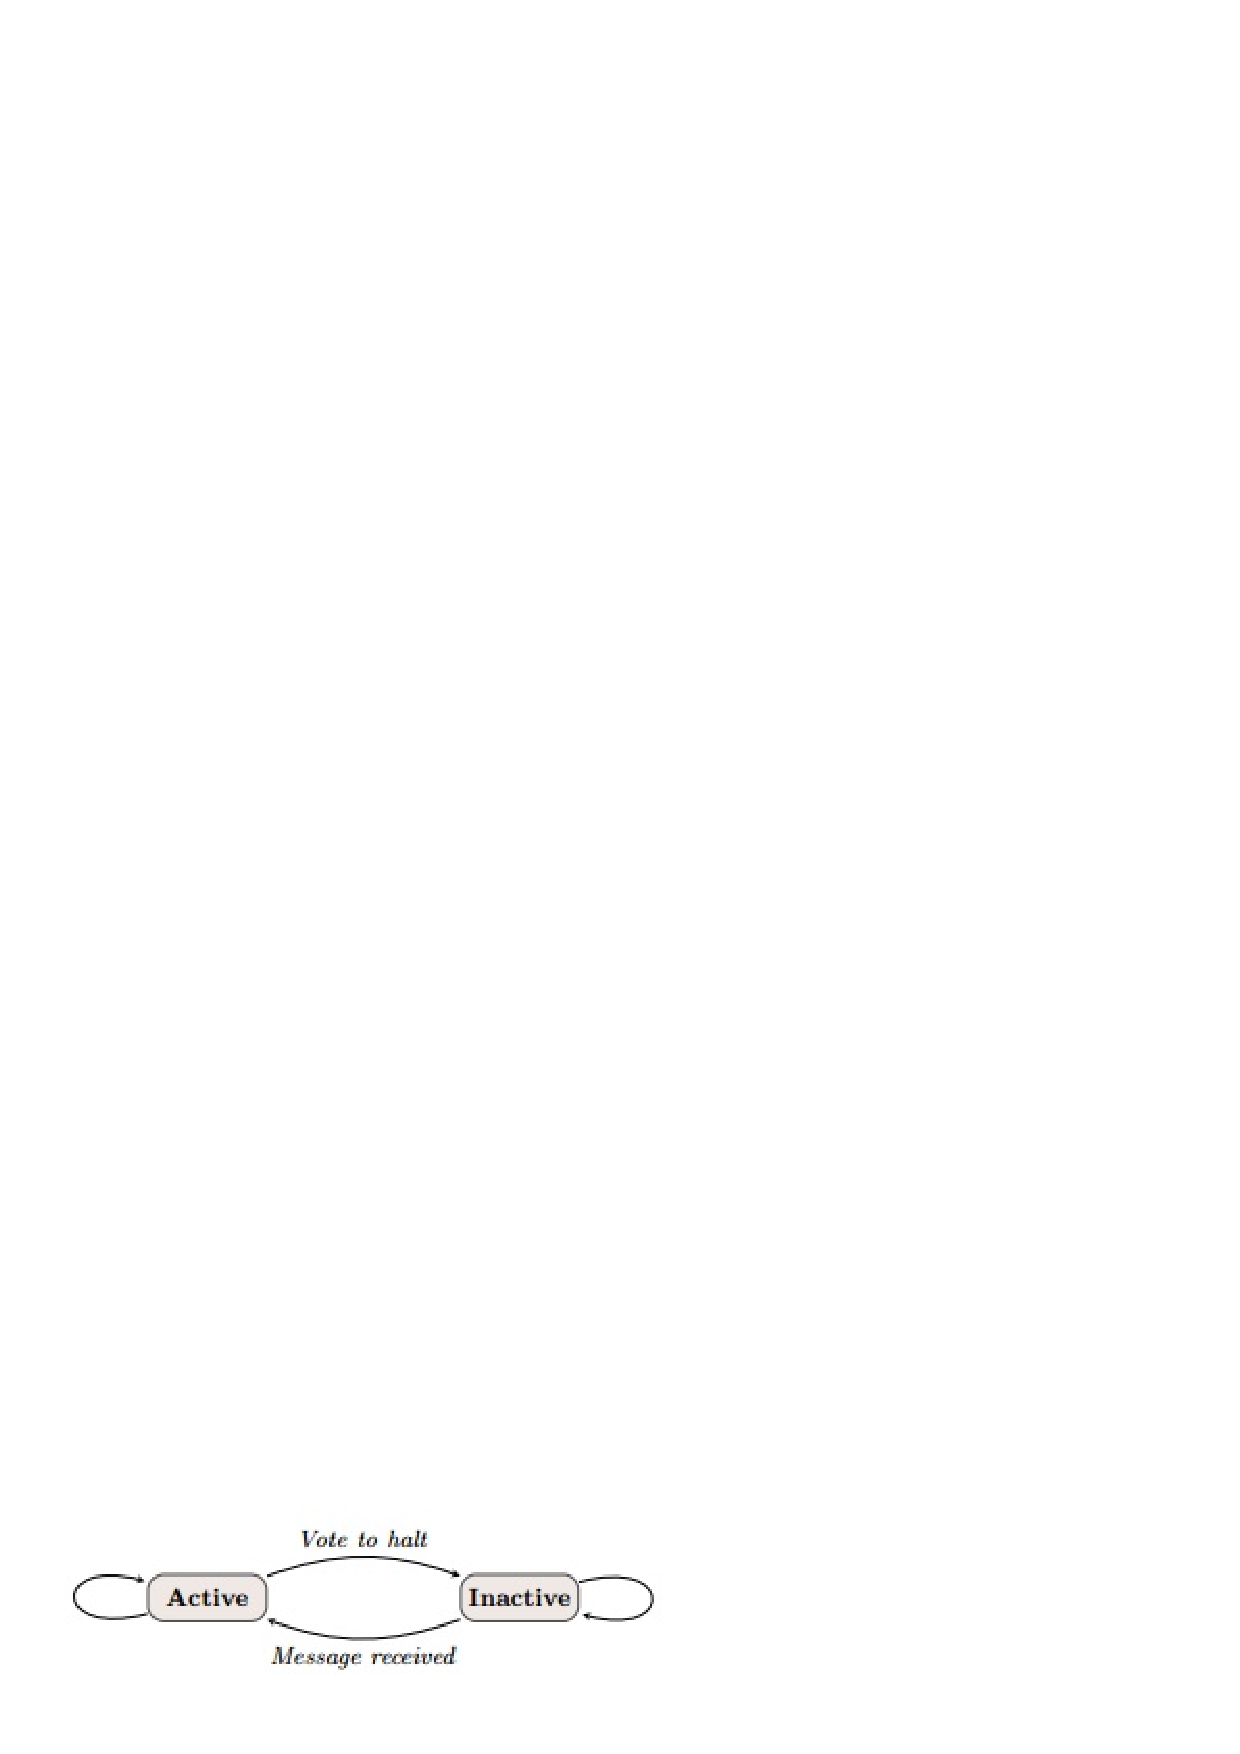
\includegraphics[width=\linewidth]{pic/vertex_state_machine}
\caption{Vertex State Machine}
\label{fig_vertex_state_machine}
\end{figure}

MapReduce can do what Pregel does but it is much more complicated to program. Each superstep can be treated as one MapReduce operation. However, Pregel is easier because the communication overhead is smaller than MapReduce which passes all the state from one iteration to next. 


\section{The C++ API}
The implementation consists of creating a \textit{Vertex} class in C++. The user needs to write a Compute() method. This method is the user specified function for each vertex and will therefore be run within each superstep. Compute() can look up vertex's value by calling GetValue() and modify the vertex's value by invoking MutableValue(). As for the value for attached edges, the vertex can change their value by calling GetOutEdgeIterator(). All state changes caused by above mentioned functions take effects immediately for all these options are locally constrained. 

\subsubsection{Message Passing}
Each vertex can communicate with other vertices by sending messages. A vertex can send any number of messages within a superstep. The message type is specified by user in the Vertex class. 

Messages sent in superstep $S$ are guaranteed to arrive at designated vertex in superstep $S+1$. The order of message may not be assured but there will be no duplication of messages.  

When there is no such destination vertex, a user defined function will be invoked to handle this exception. 

\subsubsection{Combiners}
For some graph algorithms, overall message sent between vertices could be dramatically reduced with the help from users. This is achieved through a Combine() method provided to user. For instance, when a vertex receives multiple messages containing only integers and only the sum of these integers matter. Then Pregel can combine all these integers into their sum so that reduce the communication workload to sending one message containing only the resulting sum. However, this is not enabled by default for only commutative and associative operation can be used for Combiners. 

\subsubsection{Aggregators}
This is the mechanism Pregel provides for global communication. Very much like global variable. Within each superstep $S$, each vertex can provide a value to an aggregator, Pregel will use a reduction operator to produce a sum which is going to be used for the $S+1$ superstep. Aggregators should be both commutative and associative. 

\subsubsection{Topology Mutations}
Algorithms like minimum spanning tree can change the topology by removing edges from the starting graph. This sort of modification to the graph is achieved through Compute() function too. A vertex can only delete itself and its outgoing edges. 

\subsection{Implementation}
Pregel was designed for Google clusters. Clusters consists of commodity PCs interconnected with high bandwidth.  

\subsubsection{Basic architecture}
A graph is partitioned into different regions. Each region is consisting of a set of vertices and their edges. This partition is solely based on vertex identifiers. This is equivalent to saying that we know in advance which region a particular vertex belongs to. Even if some vertex has not yet existed. This partition process can be replaced by user defined process. For example user can design a process in which close vertices are assigned to same machine. 

Typical execution of Pregel is like the following:
\begin{itemize}
    \item Pregel runs on a cluster of machines. Every machine runs the same copy of the program. One one them is assigned to be the master and others workers. Workers will resolve the position of the master and sends message to the master. The master is not assigned to any region of the graph. It just sits there and coordinate all the workers.
    \item The master decides how many regions there should be and assign vertices to machines. Allow multiple regions on one worker usually increases parallelism. 
    \item The master assigned portion of inputs to workers. Usually the input is decomposed into portions based on file boundaries, which has noting to do with the partition of graph. Therefore workers can read in input portions that does not belong to its region. When input belongs to the workers regtion, its part of region is updated immediately, otherwise when the input portion belongs to other workers, messages to designated worker will be sent. When input finalizes, all vertices are marked active  
    \item The master tell workers to start superstep. Terminate until all vertices are inactive and no messages in transit 
    \item Upon termination, the master tells the workers to save the result. 
\end{itemize}

\subsubsection{Fault tolerance}
Because commodity PCs are used as the computing cluster. It is very likely some workers will break down during execution. This break down is to be determined using a "pinging" technique. With a fixed interval of execution time, the master sends a ping message to workers. If a worker does not receive a message for some course of time, it terminates its process. If the master does not hear back form some worker for a fixed amount of time, the master mark the worker as down.  

When failure happens, the master reload the graph region that fails to the start of the current superstep and redo all the computation from there. 


% An example of a floating figure using the graphicx package.
% Note that \label must occur AFTER (or within) \caption.
% For figures, \caption should occur after the \includegraphics.
% Note that IEEEtran v1.7 and later has special internal code that
% is designed to preserve the operation of \label within \caption
% even when the captionsoff option is in effect. However, because
% of issues like this, it may be the safest practice to put all your
% \label just after \caption rather than within \caption{}.
%
% Reminder: the "draftcls" or "draftclsnofoot", not "draft", class
% option should be used if it is desired that the figures are to be
% displayed while in draft mode.
%
%\begin{figure}[!t]
%\centering
%\includegraphics[width=2.5in]{myfigure}
% where an .eps filename suffix will be assumed under latex, 
% and a .pdf suffix will be assumed for pdflatex; or what has been declared
% via \DeclareGraphicsExtensions.
%\caption{Simulation Results.}
%\label{fig_sim}
%\end{figure}

% Note that IEEE typically puts floats only at the top, even when this
% results in a large percentage of a column being occupied by floats.


% An example of a double column floating figure using two subfigures.
% (The subfig.sty package must be loaded for this to work.)
% The subfigure \label commands are set within each subfloat command,
% and the \label for the overall figure must come after \caption.
% \hfil is used as a separator to get equal spacing.
% Watch out that the combined width of all the subfigures on a 
% line do not exceed the text width or a line break will occur.
%
%\begin{figure*}[!t]
%\centering
%\subfloat[Case I]{\includegraphics[width=2.5in]{box}%
%\label{fig_first_case}}
%\hfil
%\subfloat[Case II]{\includegraphics[width=2.5in]{box}%
%\label{fig_second_case}}
%\caption{Simulation results.}
%\label{fig_sim}
%\end{figure*}
%
% Note that often IEEE papers with subfigures do not employ subfigure
% captions (using the optional argument to \subfloat[]), but instead will
% reference/describe all of them (a), (b), etc., within the main caption.


% An example of a floating table. Note that, for IEEE style tables, the 
% \caption command should come BEFORE the table. Table text will default to
% \footnotesize as IEEE normally uses this smaller font for tables.
% The \label must come after \caption as always.
%
%\begin{table}[!t]
%% increase table row spacing, adjust to taste
%\renewcommand{\arraystretch}{1.3}
% if using array.sty, it might be a good idea to tweak the value of
% \extrarowheight as needed to properly center the text within the cells
%\caption{An Example of a Table}
%\label{table_example}
%\centering
%% Some packages, such as MDW tools, offer better commands for making tables
%% than the plain LaTeX2e tabular which is used here.
%\begin{tabular}{|c||c|}
%\hline
%One & Two\\
%\hline
%Three & Four\\
%\hline
%\end{tabular}
%\end{table}


% Note that IEEE does not put floats in the very first column - or typically
% anywhere on the first page for that matter. Also, in-text middle ("here")
% positioning is not used. Most IEEE journals/conferences use top floats
% exclusively. Note that, LaTeX2e, unlike IEEE journals/conferences, places
% footnotes above bottom floats. This can be corrected via the \fnbelowfloat
% command of the stfloats package.

% trigger a \newpage just before the given reference
% number - used to balance the columns on the last page
% adjust value as needed - may need to be readjusted if
% the document is modified later
%\IEEEtriggeratref{8}
% The "triggered" command can be changed if desired:
%\IEEEtriggercmd{\enlargethispage{-5in}}

% references section

% can use a bibliography generated by BibTeX as a .bbl file
% BibTeX documentation can be easily obtained at:
% http://www.ctan.org/tex-archive/biblio/bibtex/contrib/doc/
% The IEEEtran BibTeX style support page is at:
% http://www.michaelshell.org/tex/ieeetran/bibtex/
%\bibliographystyle{IEEEtran}
% argument is your BibTeX string definitions and bibliography database(s)
%\bibliography{IEEEabrv,../bib/paper}
%
% <OR> manually copy in the resultant .bbl file
% set second argument of \begin to the number of references
% (used to reserve space for the reference number labels box)
%\begin{thebibliography}{1}
%
%\bibitem{IEEEhowto:kopka}
%H.~Kopka and P.~W. Daly, \emph{A Guide to \LaTeX}, 3rd~ed.\hskip 1em plus
%  0.5em minus 0.4em\relax Harlow, England: Addison-Wesley, 1999.
%
%\end{thebibliography}
\bibliography{pregel_citation}
\bibliographystyle{plain}
\end{document}


